
\documentclass[a4paper,12pt]{article}
\usepackage[pdftex, hidelinks]{hyperref}

\usepackage{bm}
\usepackage[T1]{fontenc}
\usepackage[utf8]{inputenc}
\usepackage{algorithmic}
\usepackage{algorithm}
\usepackage{amsfonts}
\usepackage{amssymb}
\usepackage{courier}
\usepackage{booktabs}
\usepackage{graphicx}
\usepackage{listings}
\usepackage{mathtools}
\usepackage{amssymb}
\lstset{
language=R,
basicstyle=\ttfamily
}

\title{TDDE01 -- Machine Learning \\
Individual Lab Report 4}
\author{Martin Estgren \texttt{<mares480>}}

\begin{document}
\pagenumbering{arabic}
    \maketitle % Generate.
    \section{Assignment 1}
    In this assignment we will be analyzing the \textit{percentage of population living in standard metropolitan areas} (MET) over the \textit{Per capita state and local public expenditures} (EX) by using \textit{regression trees}. 

    We first plot the data (as seen in figure~\ref{fig:A1_data}) and examine what kind of model could be of interest. 

    \begin{figure}[H]
    \centering
    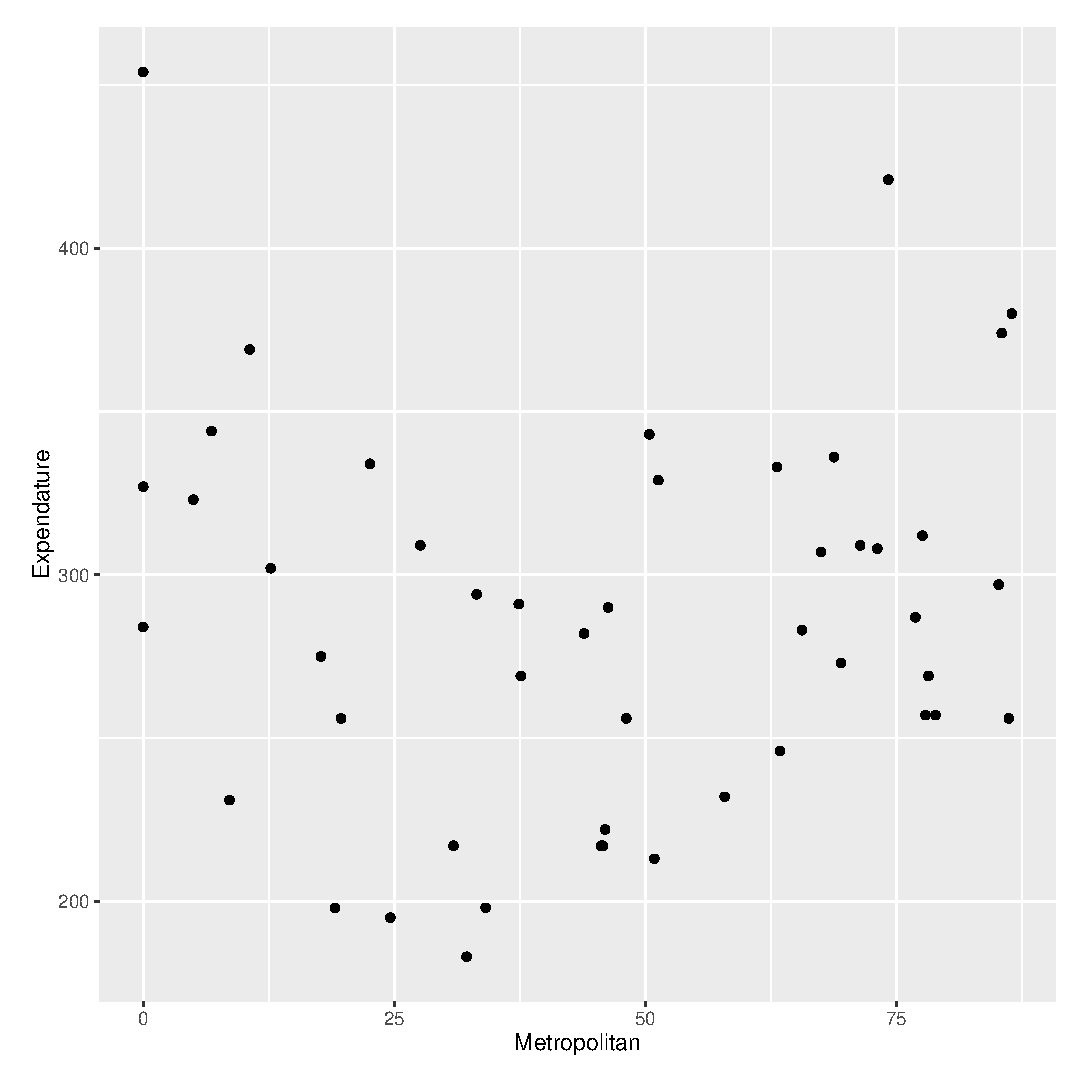
\includegraphics[width=\textwidth]{figures/A1_data}  
    \caption{Raw data plot. \label{fig:A1_data}}
    \end{figure}


    There is no observable pattern of significance in the figure. But a \textit{tree model} would probably be a better model than \textit{linear regression}. Because the response variable is continuous we decide on a \textit{regression tree mode}. 

    The \textit{regression tree mode} we decide on will use \textit{cross validation} and the minimal number of observations in each leaf to 8. The resulting tree can be seen inf figure~\ref{fig:A1_tree}.

    \begin{figure}[H]
    \centering
    \includegraphics[width=\textwidth]{figures/A1_tree}  
    \caption{Optimal regression tree model \label{fig:A1_tree}}
    \end{figure}
    The optimal tree model resulted in three leafs. The model predictions can be seen in figure~\ref{fig:A1_fit} and a histogram of residuals in figure~\ref{fig:A1_historgram_residuals}.

    \begin{figure}[H]
    \centering
    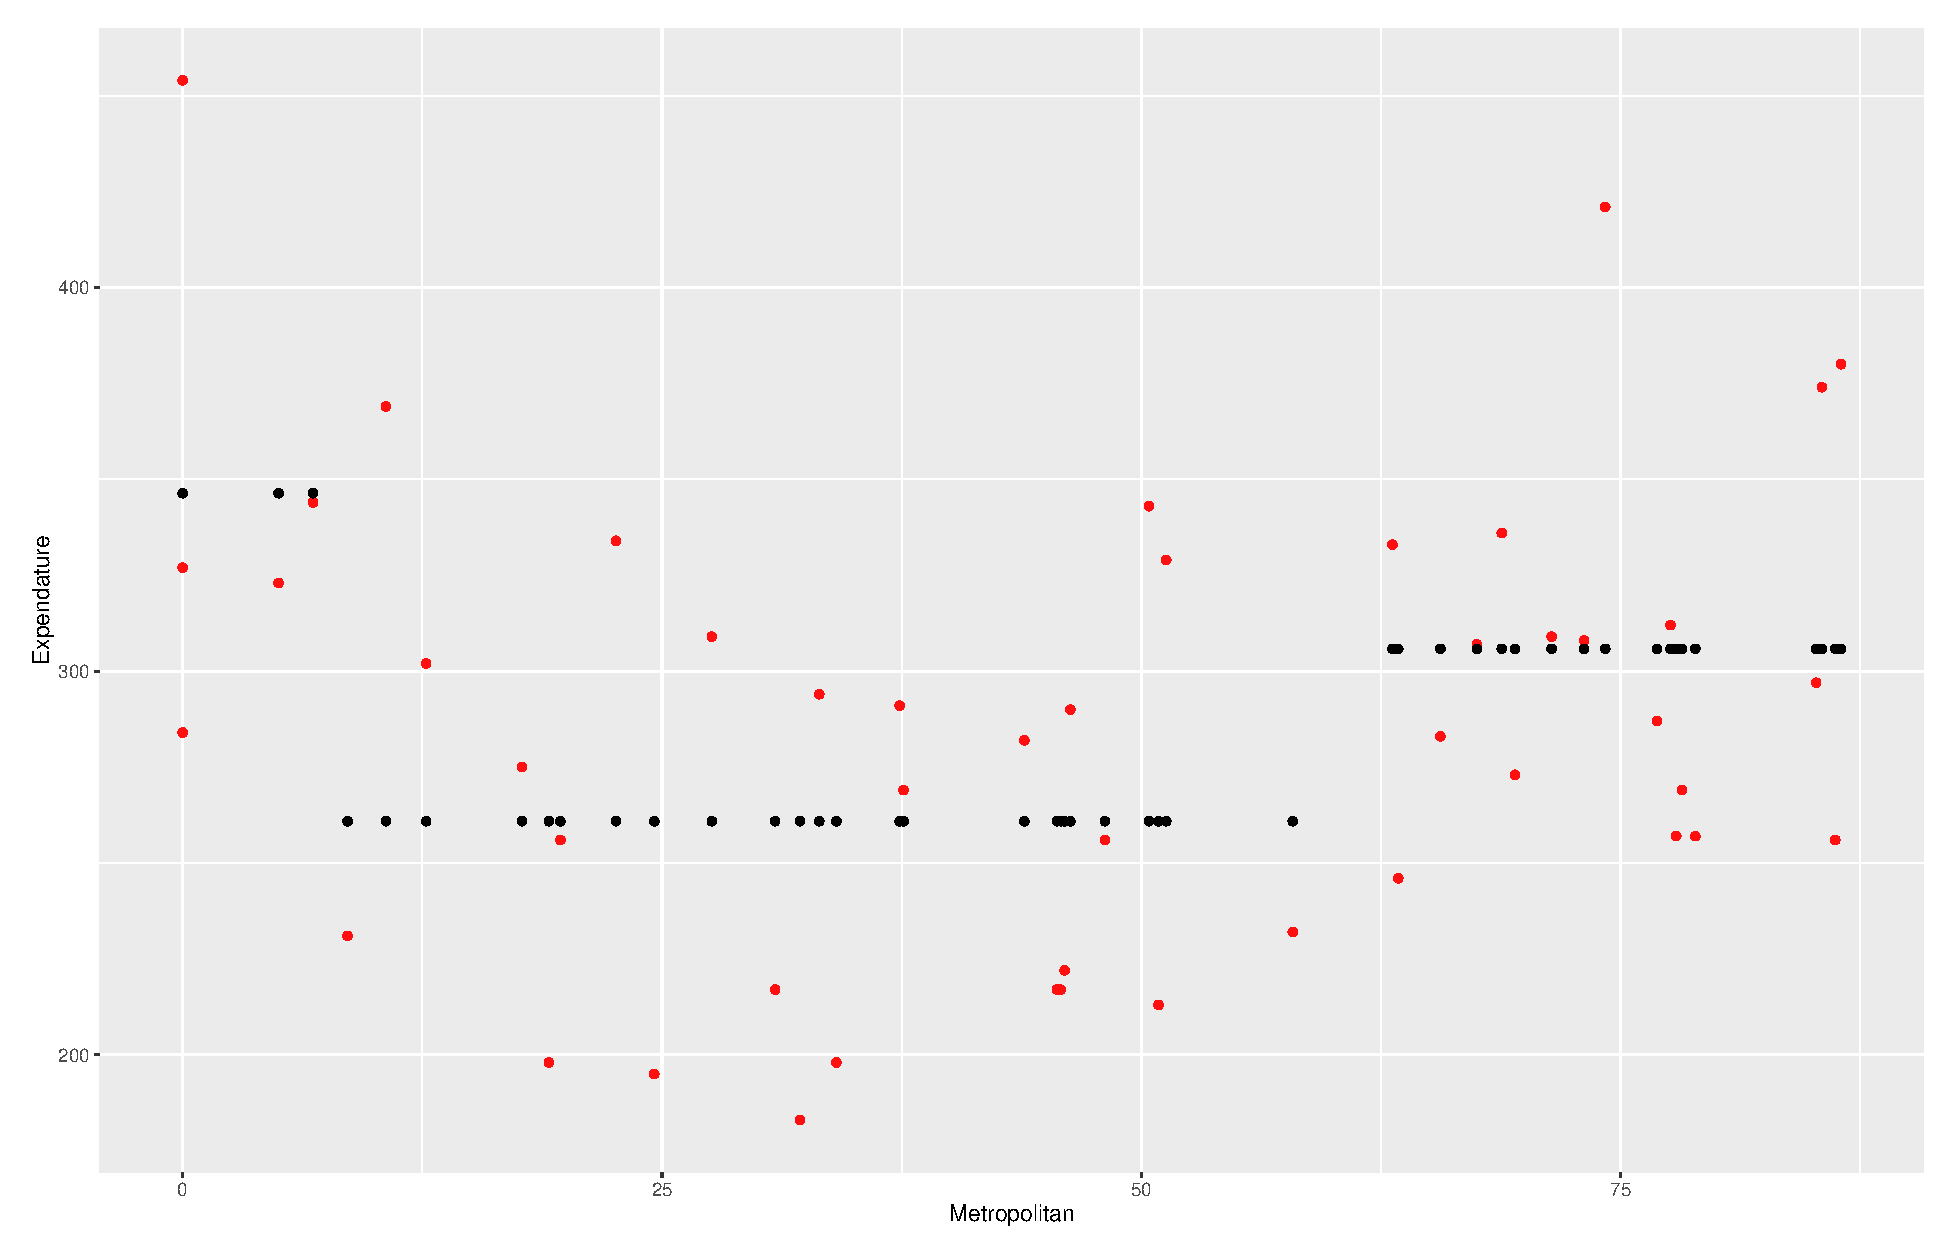
\includegraphics[width=\textwidth]{figures/A1_fit}  
    \caption{Predictions of the tree model \label{fig:A1_fit}}
    \end{figure}
    The number of labels (3) produced by the model is significantly less than the raw data. The labels seems to be located around the respective means of the raw data. 

    \begin{figure}[H]

    \centering
    \includegraphics[width=\textwidth]{figures/A1_historgram_residuals}  
    \caption{Histogram of the model residuals \label{fig:A1_historgram_residuals}}
    \end{figure}
    Ideally, the histogram would show a normal distribution of residuals with a mean of 0. This is not what can be deduced from the model, although 48 observations are very few observations for a normal distribution to be observable with.

    To mitigate this problem we use \textit{bootstrapping} on the optimal tree model. We first try \textit{non-parametric bootstrapping}. The result is plotted with a confidence level of 0.95 in figure ~\ref{fig:A1_nonparametric}

    \begin{figure}[H]
    \centering
    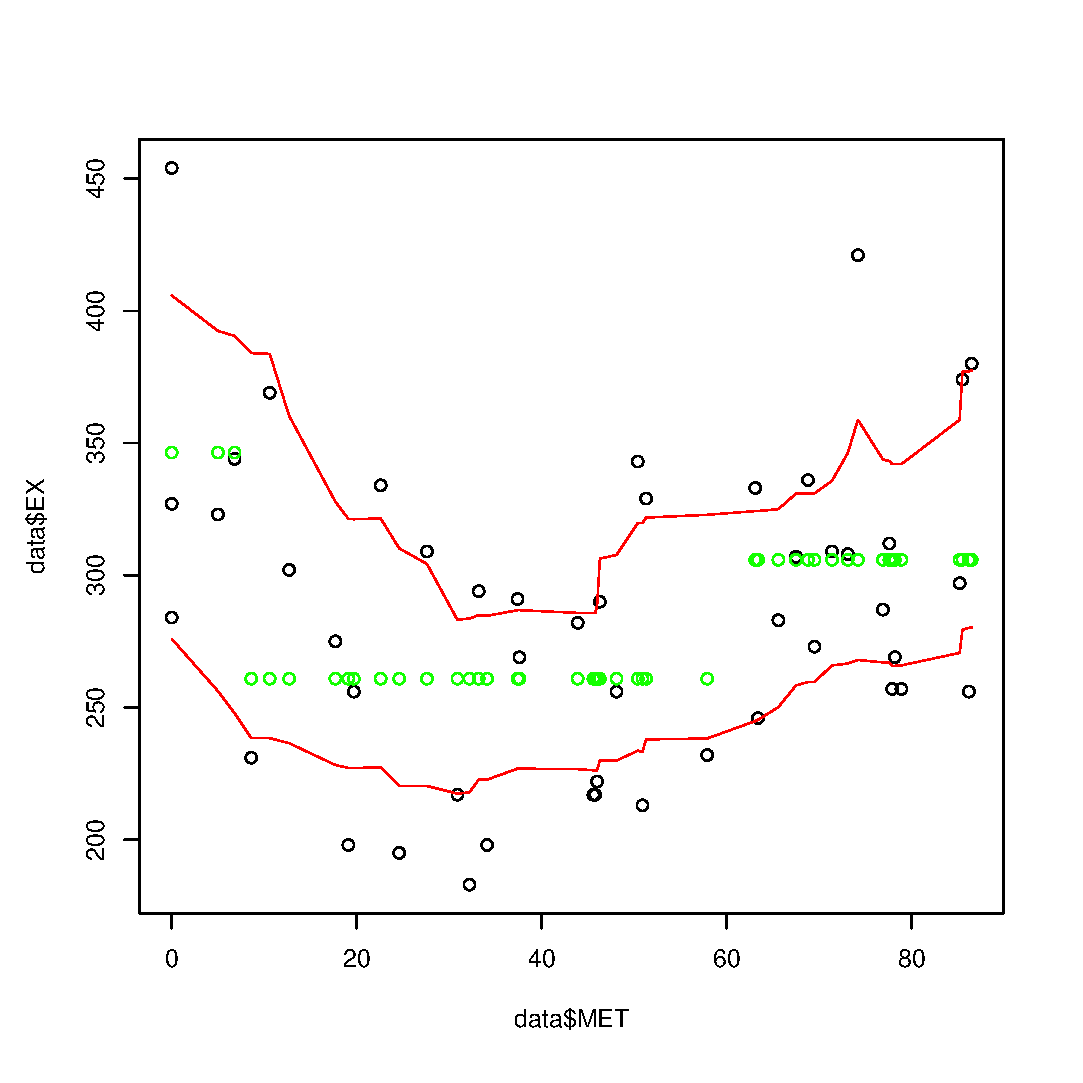
\includegraphics[width=\textwidth]{figures/A1_nonparametric}  
    \caption{0.95 confidence bound of the non-parametric bootstrap. \label{fig:A1_nonparametric}}
    \end{figure}
    We can observe how most of the observations are located within the confidence bound but significantly more than 0.05 still outside. The result would indicate that the tree model isn't a perfect fit for the data.

    We examine the same model, this time using \textit{parametric bootstrap} where we assume the observations fall within the distribution:
    \begin{equation}
    Y \sim  N(\mu_i,\theta^2)
    \end{equation}
    The resulting plot can be seen in the figure~\ref{fig:A1_parametric}. 

    \begin{figure}[H]
    \centering
    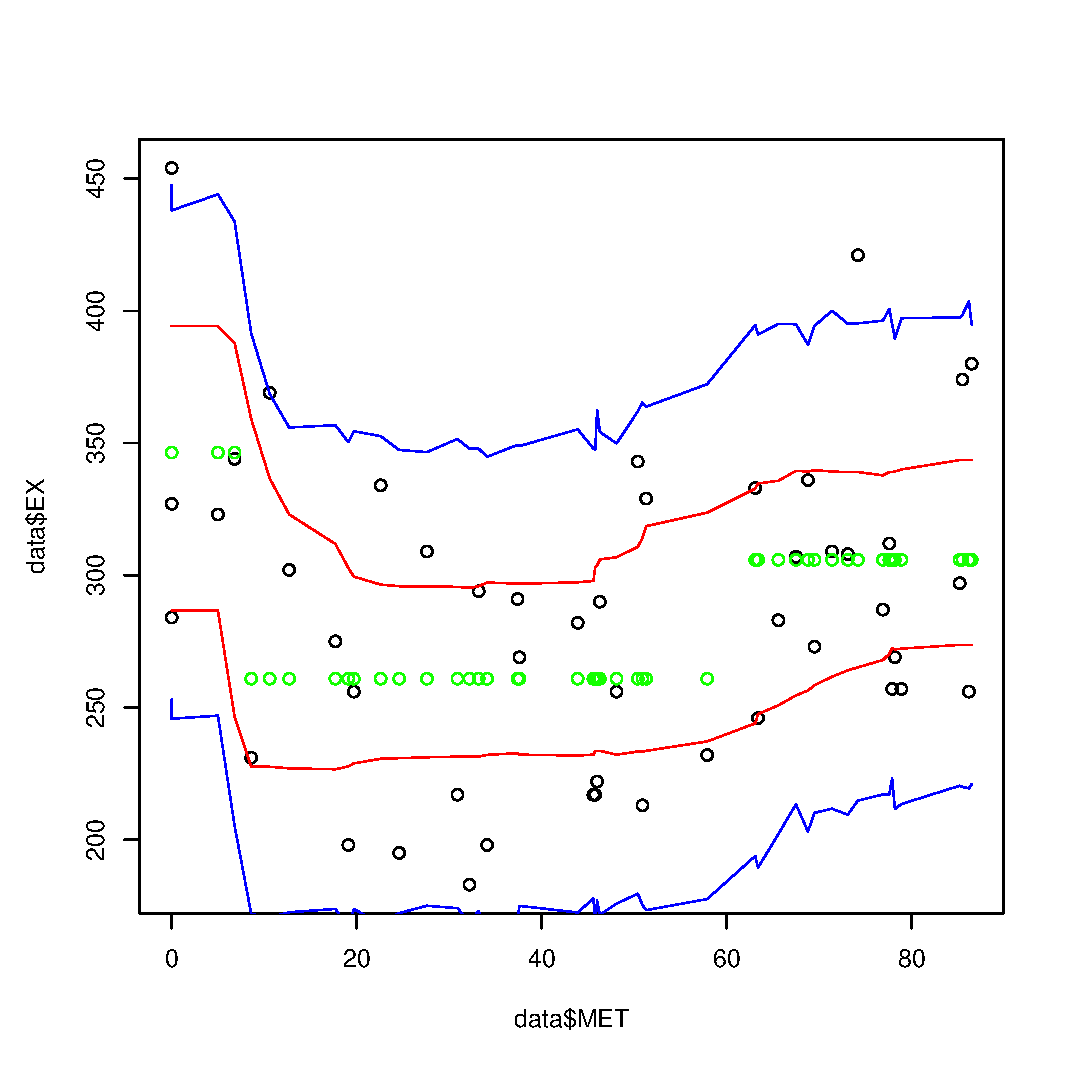
\includegraphics[width=\textwidth]{figures/A1_parametric}  
    \caption{0.95 confidence bound and predictions bound of the parametric bootstrap. \label{fig:A1_parametric}}
    \end{figure}
    The 0.95 confidence bound is much tighter around the predictions compared to the \textit{non-parametric bootstrap} with the \textit{prediction bound} encompassing all-but a few outliers of the observations. The \textit{prediction bound} can be seen as the 0.95 confidence bound of the assumed distribution. Looking back at the residuals in figure~\ref{fig:A1_historgram_residuals} we cant tell for sure if the data would follow a normal distribution.

    Comparing the \textit{non-parametric} and the \textit{parametric} bootstrap it seems like the \textit{non-parametric} would be a better fit for the given data set. 

    \section{Assignment 2}
    In this assignment we are tasked with analyzing a data set containing observations regarding different levels of \emph{viscosity} and \emph{near-infrared spectra} for many different \emph{diesel fuels} using \emph{PCA} and \emph{ICA} (\emph{Component Analysis Functions}).

    We start by centering the data around 0 and perform a \emph{principal Component Analysis (PCA)} on the data set. The result can be seen in Figure~\ref{fig:pcahist}.

    \begin{figure}[H]            \centering
    \caption{PCA histogram of variance}
    \label{fig:pcahist}
    \includegraphics[width=\textwidth]{figures/A2_pcahist.eps}
    \end{figure}

    Only two components are required to reach 99 \% cumulative variance. The components are \emph{X750 (PC1)} and \emph{X752 (PC2)}. In Figure~\ref{fig:pcascore} the score for each of the two most significant PCs are displayed.

    \begin{figure}[H]           
    \centering
    \caption{PCA score distribution}
    \label{fig:pcascore}
    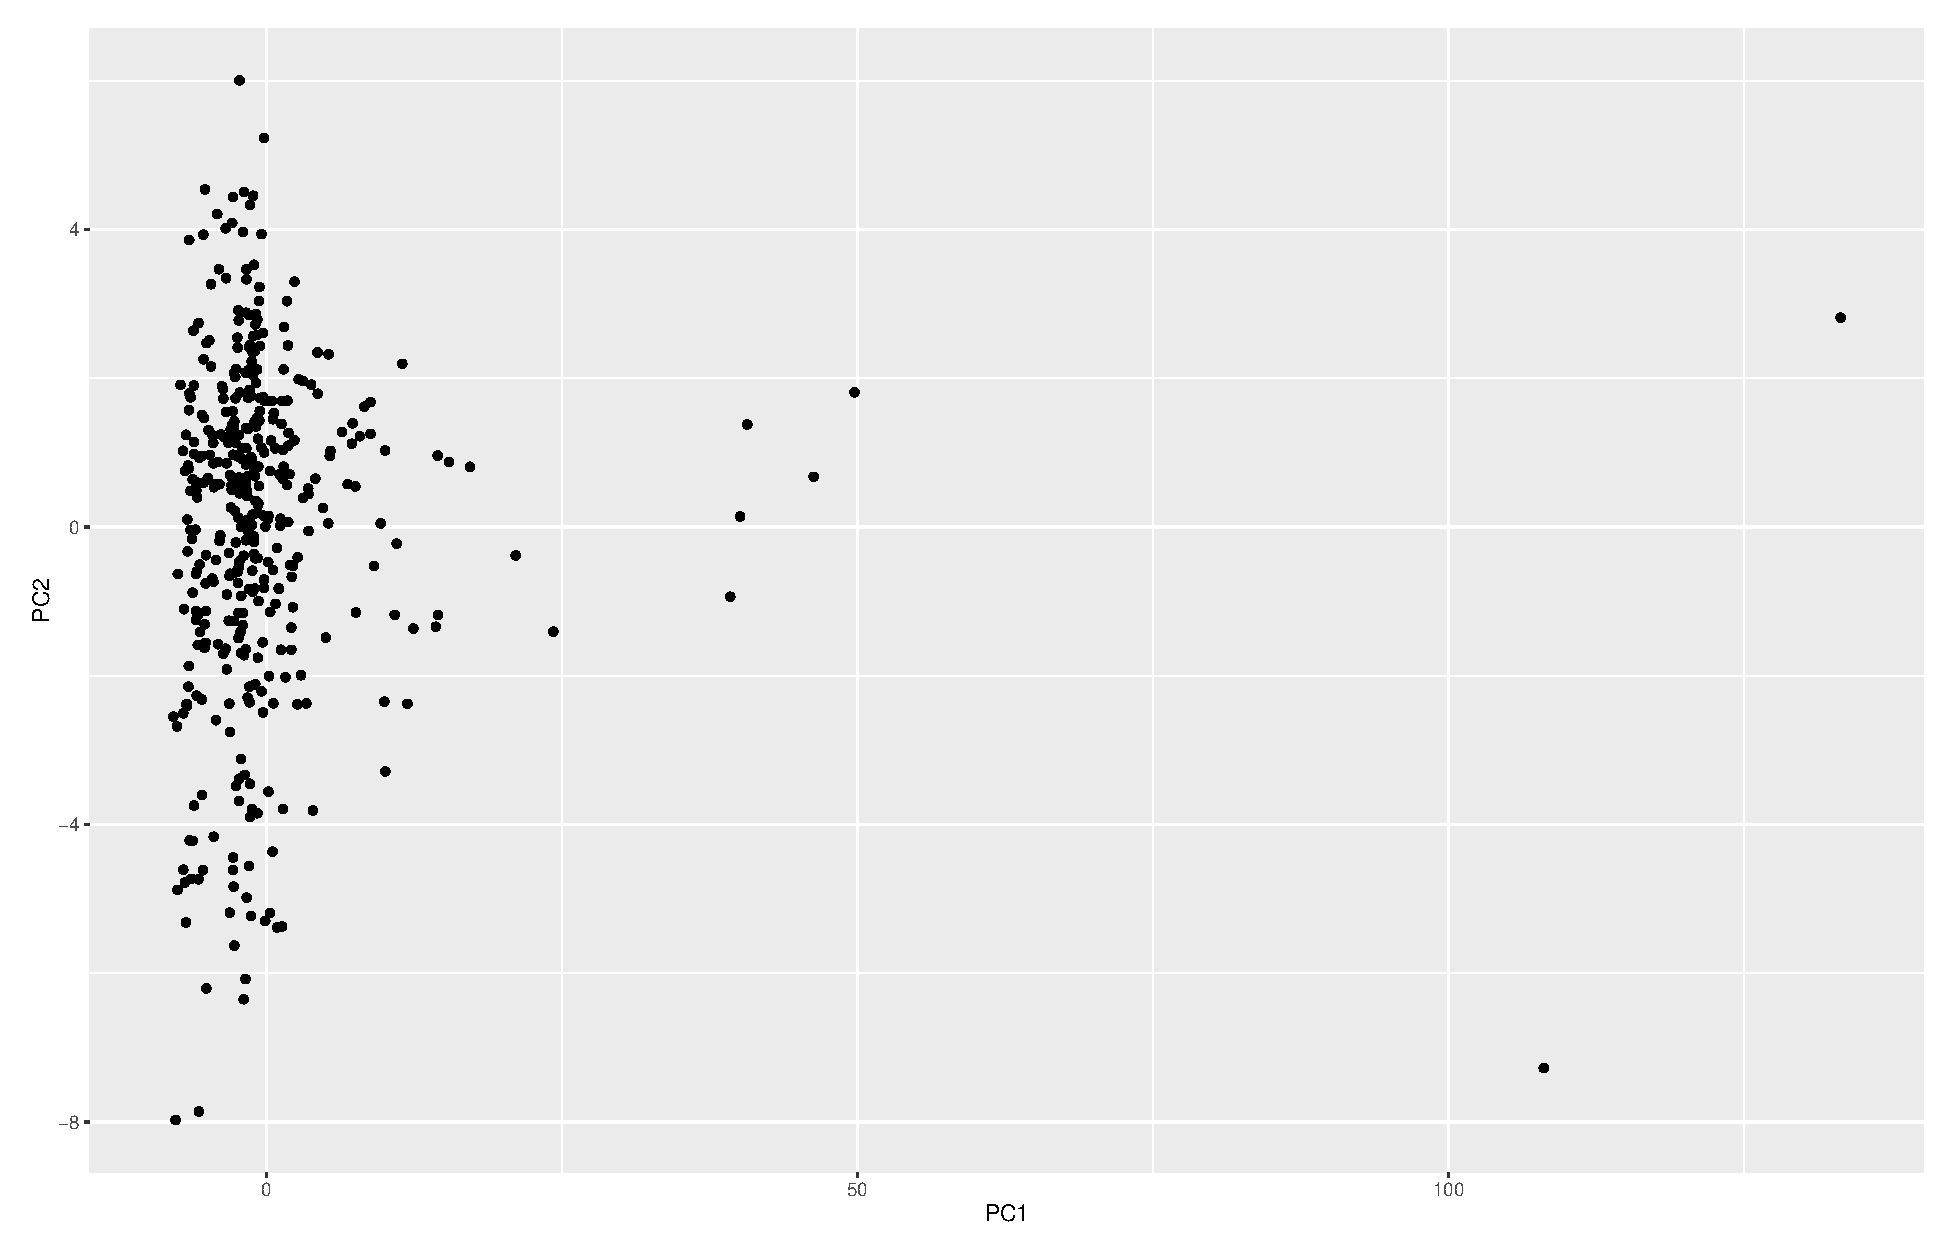
\includegraphics[width=\textwidth]{figures/A2_pcascore.eps}
    \end{figure}

    As can be seen, there is a large amount of independence between these two components on the X-axis while they are fairly compacted on the y-axis, ignoring the outliers. The outliers indicates unusual diesel fuels. We plot the traces for each of the two PCA with the highest variance impact on the variance. The resulting plots can be seen in Figures~\ref{fig:x750tp} and \ref{fig:x752tp}.
    \begin{figure}[H]      
    \centering
    \begin{minipage}[]{0.49\textwidth}
    \caption{Trace plot of PC1}
    \label{fig:x750tp}
    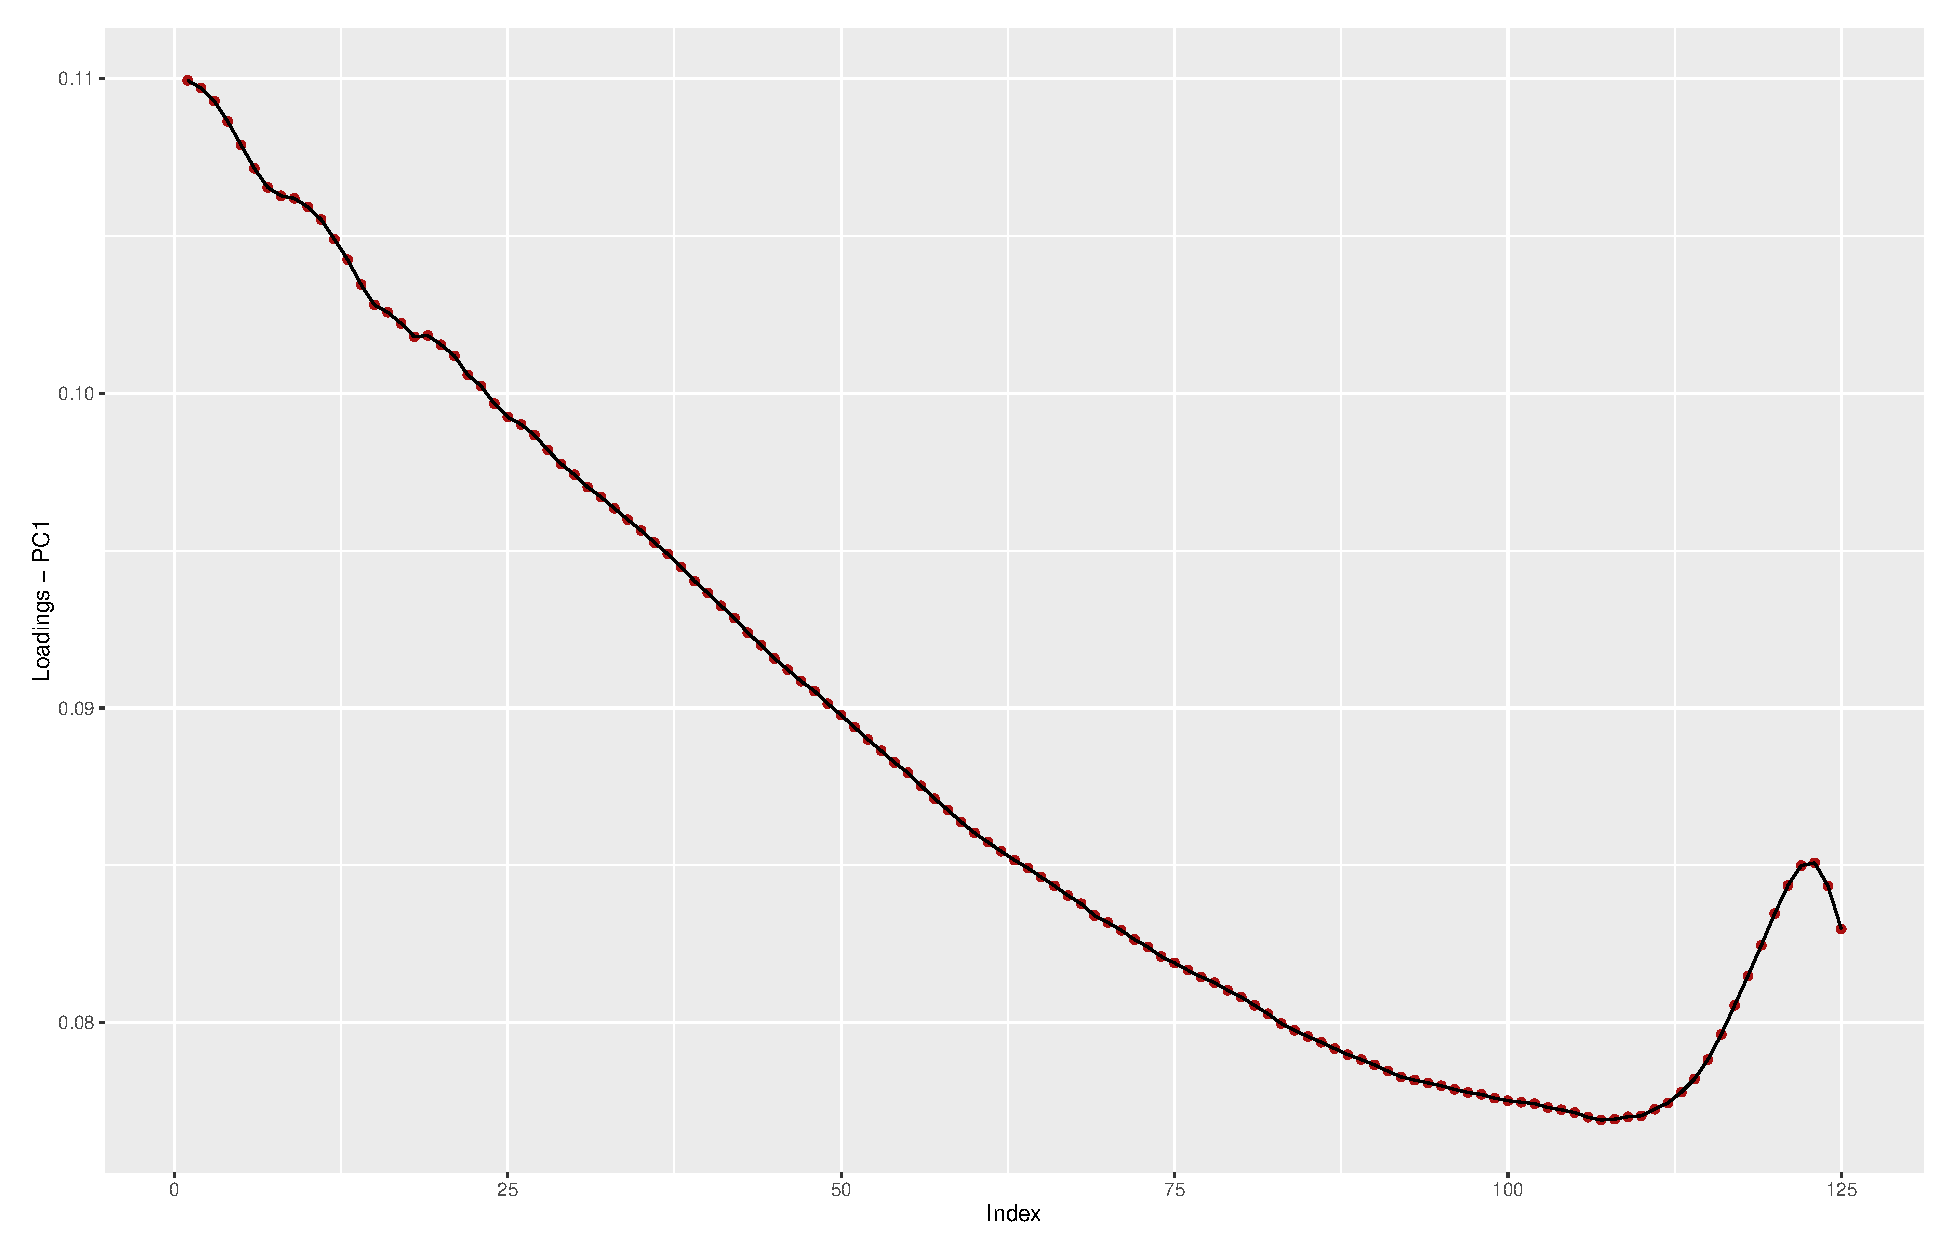
\includegraphics[width=\textwidth]{figures/A2_trace_PC1.eps}     
    \end{minipage}
    \begin{minipage}[]{0.49\textwidth}
    \caption{Trace plot of PC2}
    \label{fig:x752tp}
    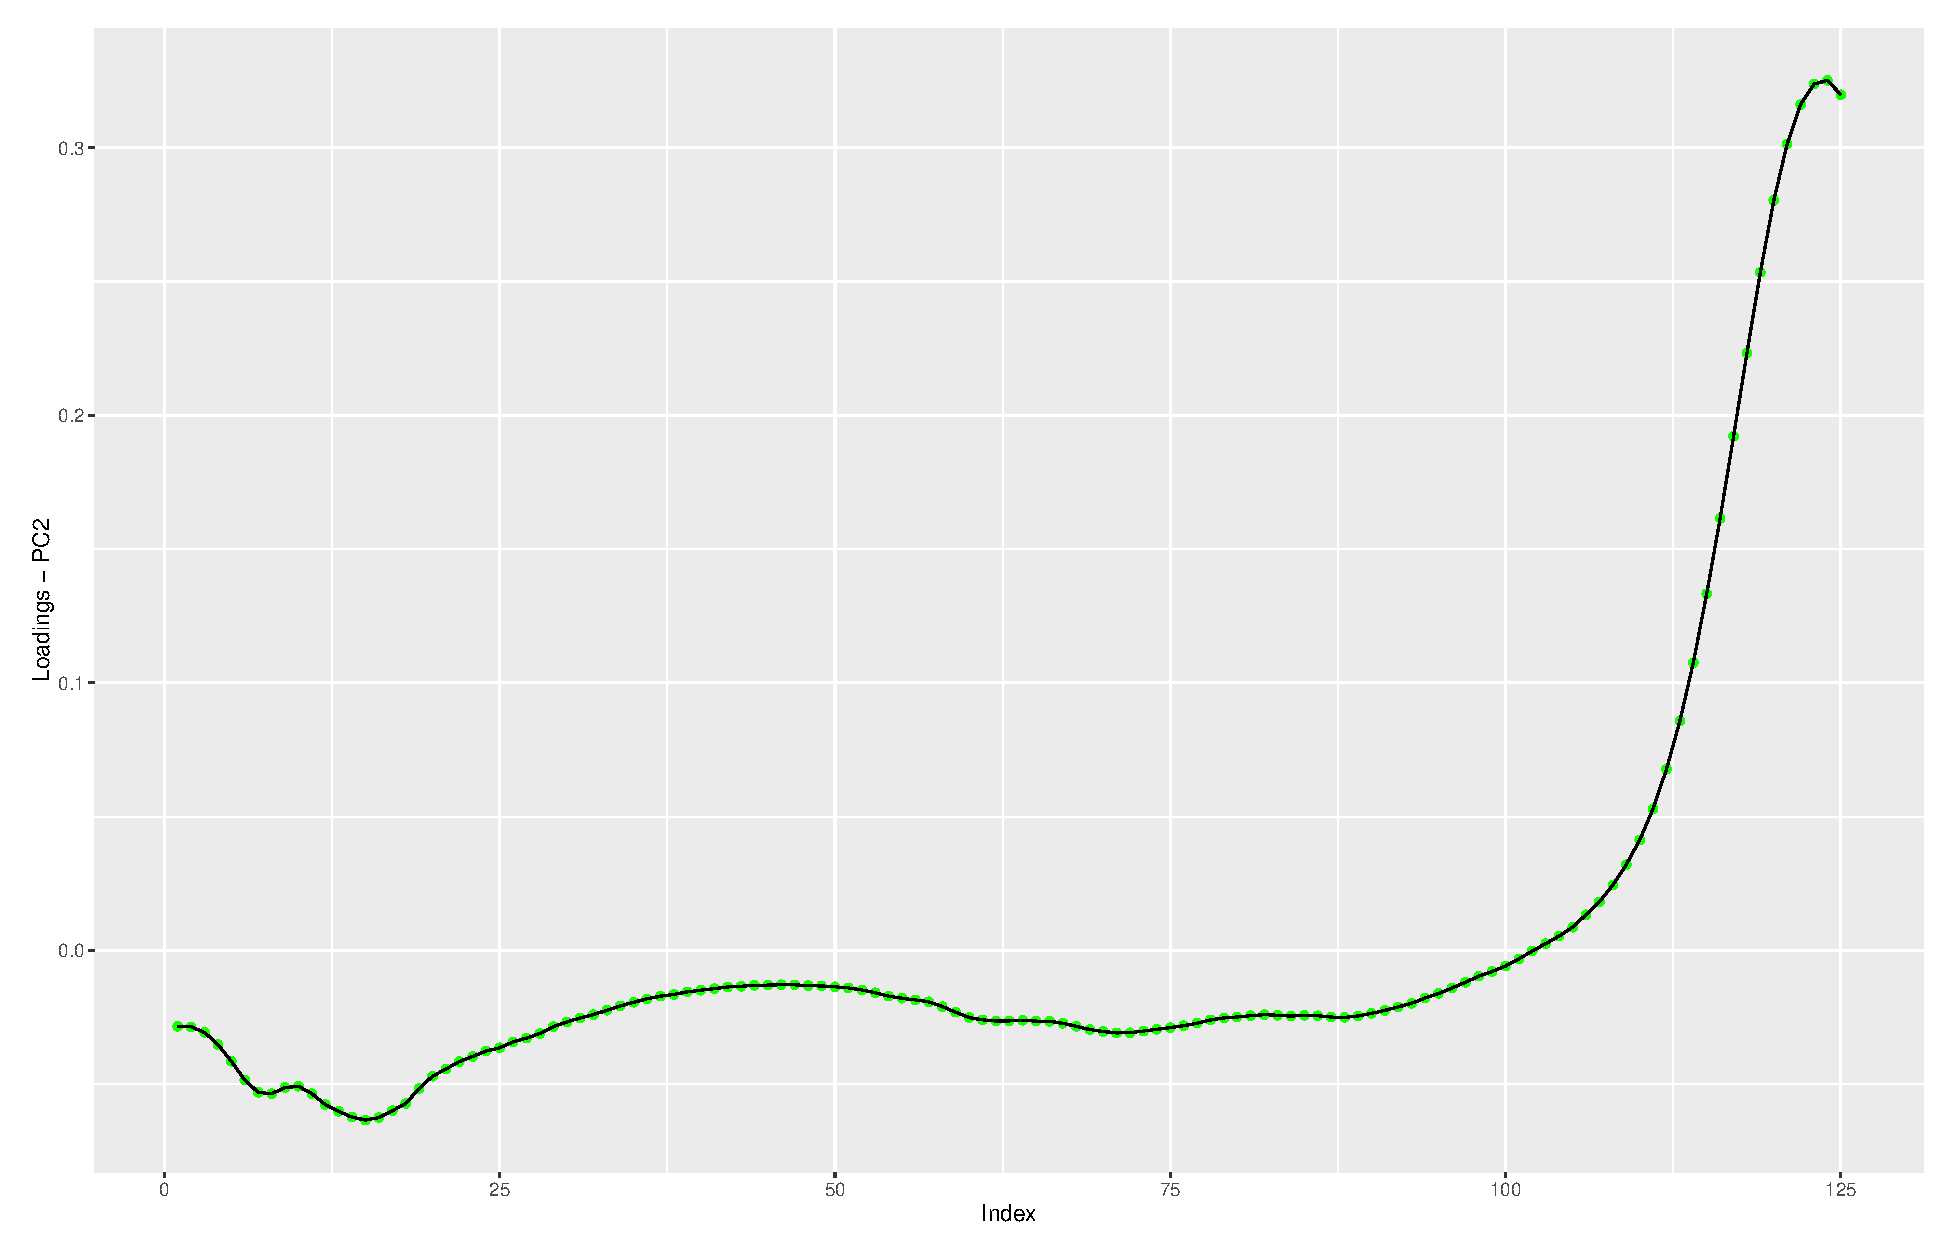
\includegraphics[width=\textwidth]{figures/A2_trace_PC2.eps}
    \end{minipage}
    \end{figure}

    We can observe how the the components where the PC1 have a high correlation, PC2 have low and vice e versa. 

    We perform the same analysis again, this time using the \emph{Independent component analysis} (ICA). In contrast to to PCA, we assume the components are independent.

    The loadings are calculated with the function \( \hat{W} = K \dot W \). The traces can be observed in Figure~\ref{fig:x750ical} and \ref{fig:x752ical}.

    \begin{figure}[H]           
    \centering
    \begin{minipage}[]{0.49\textwidth}

    \caption{Trace plot of IC1}
    \label{fig:x750ical}
    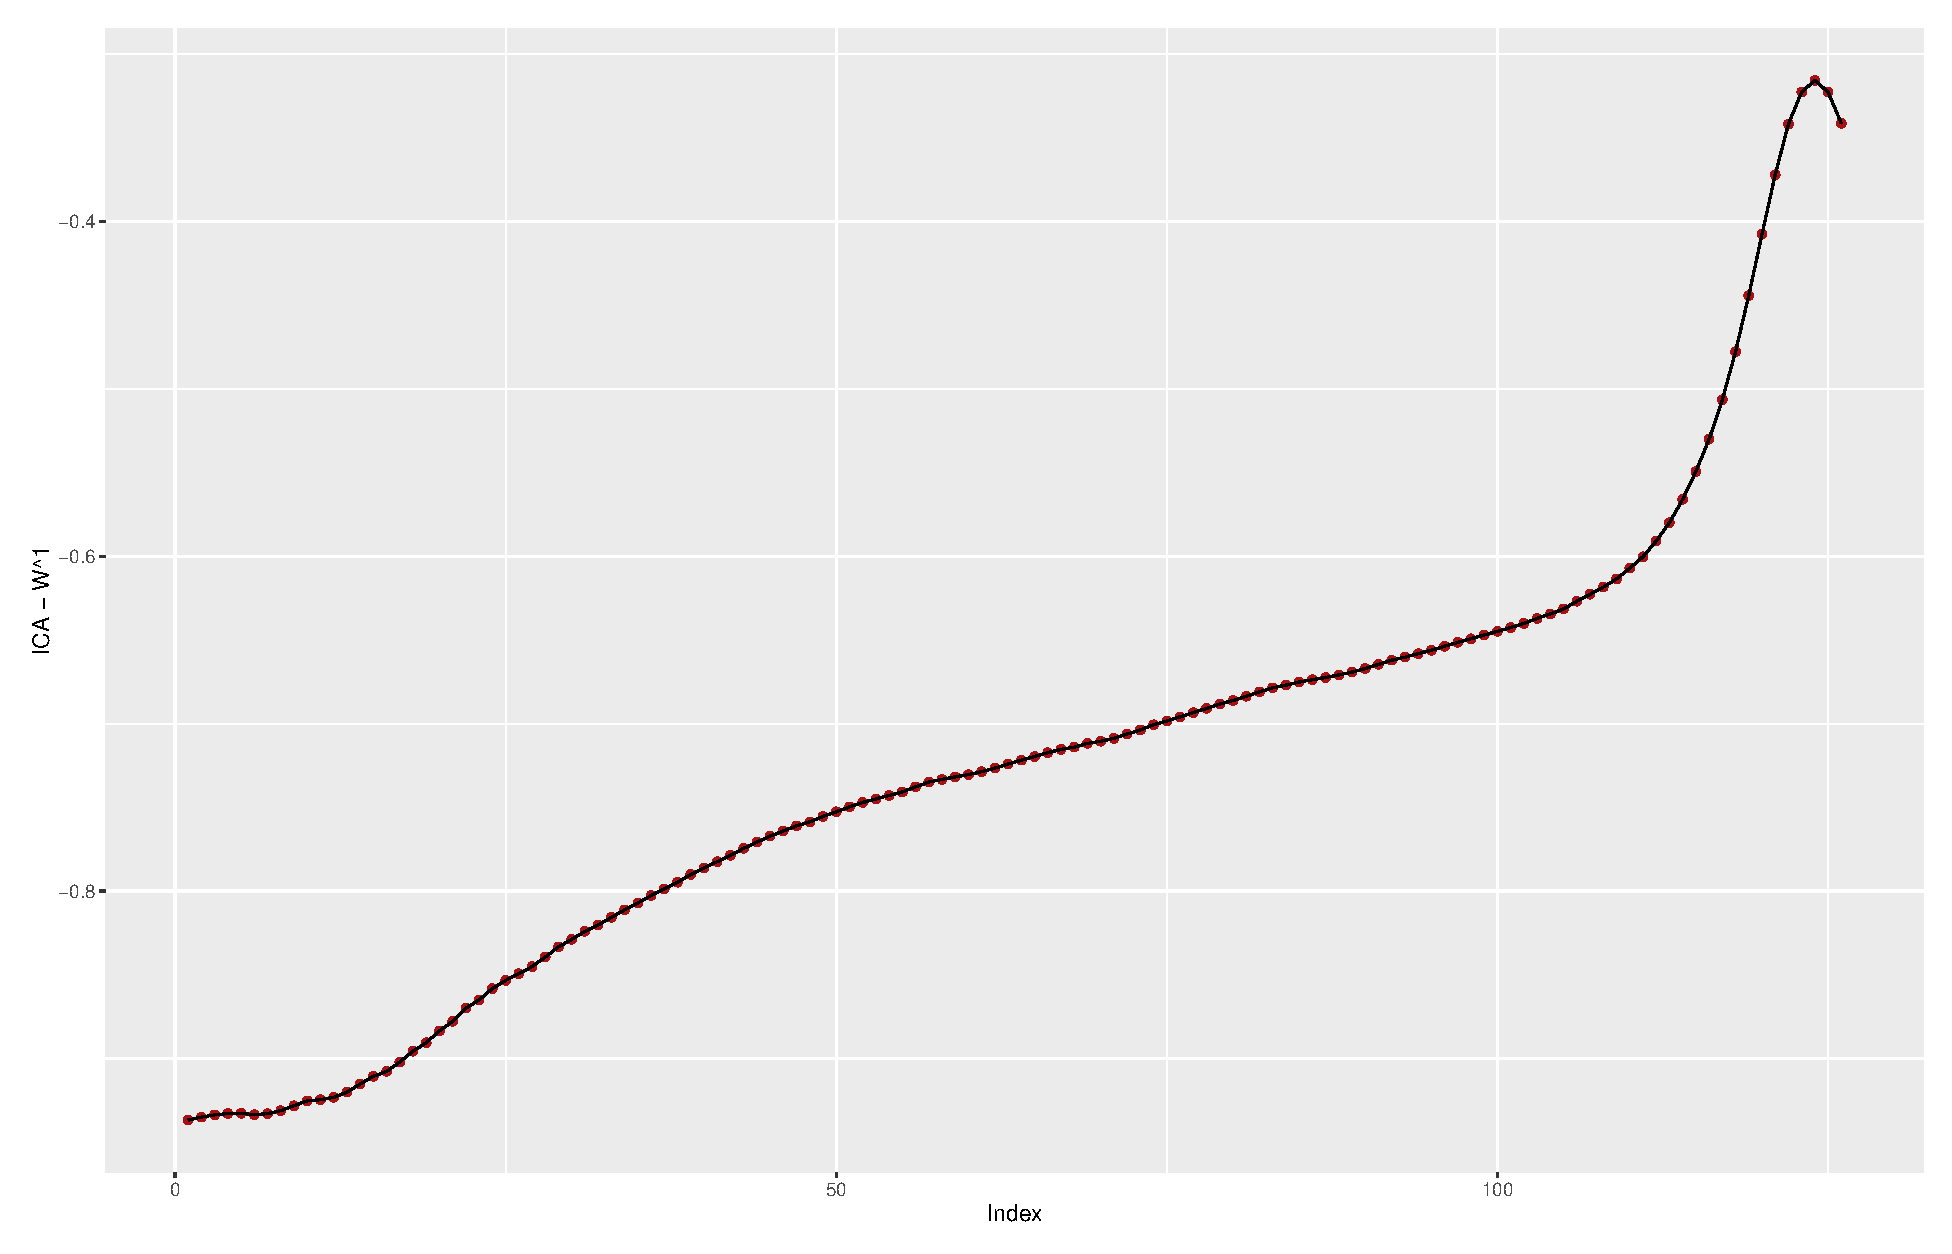
\includegraphics[width=\textwidth]{figures/A2_trace_ICA1.eps}
    \end{minipage}
    \begin{minipage}[]{0.49\textwidth}
    \caption{Trace plot of IC2}
    \label{fig:x752ical}
    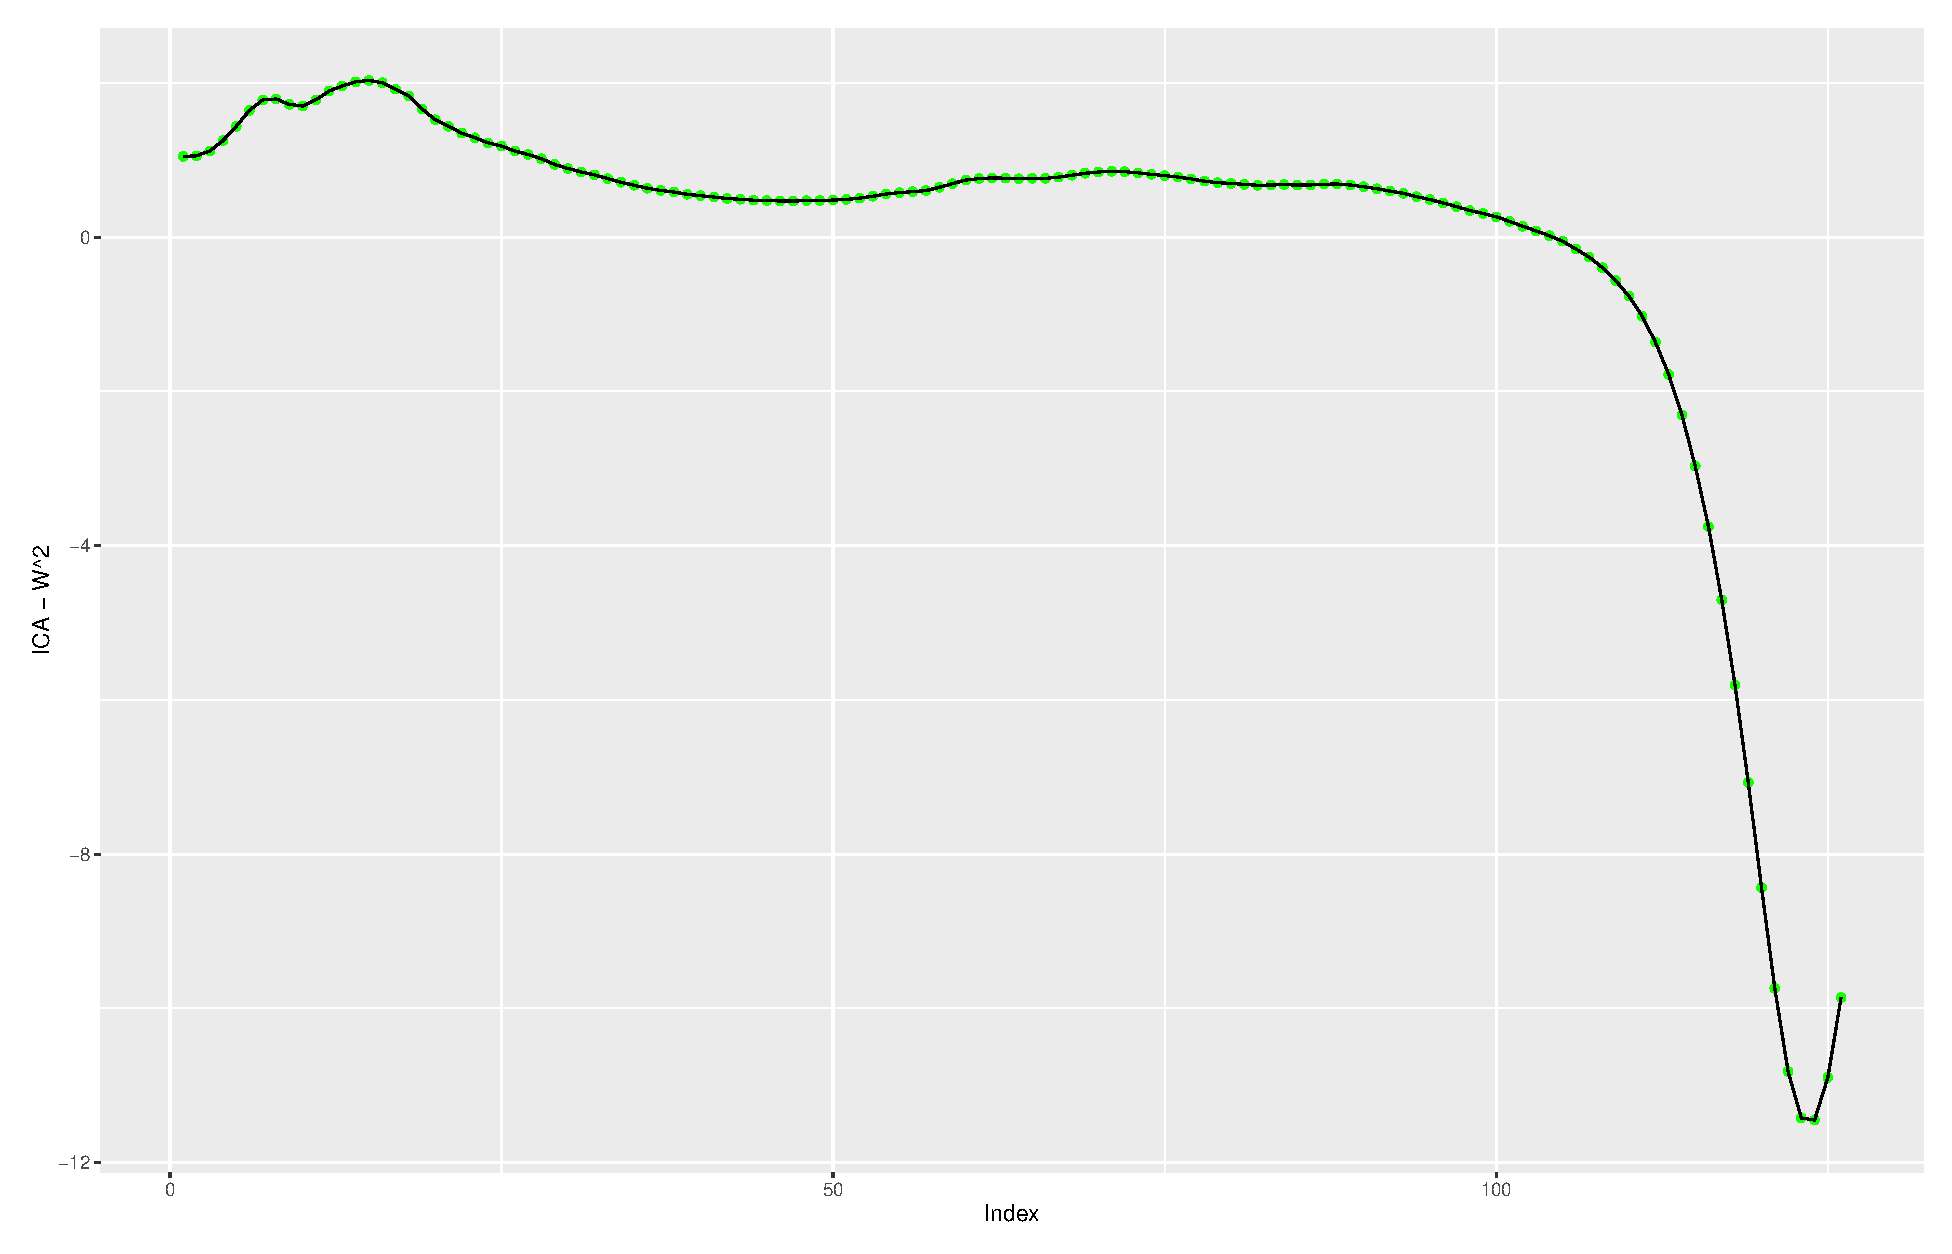
\includegraphics[width=\textwidth]{figures/A2_trace_ICA2.eps}
    \end{minipage}
    \end{figure}

    The results are quite similar to those found in PCA, but inverted. This is expected since we are looking for the independence instead of the correlation.

    We now plot the scores found by doing ICA, which can be seen in Figure~\ref{fig:icascores}.
    \begin{figure}[H]          
    \centering
    \caption{ICA score distribution}
    \label{fig:icascores}
    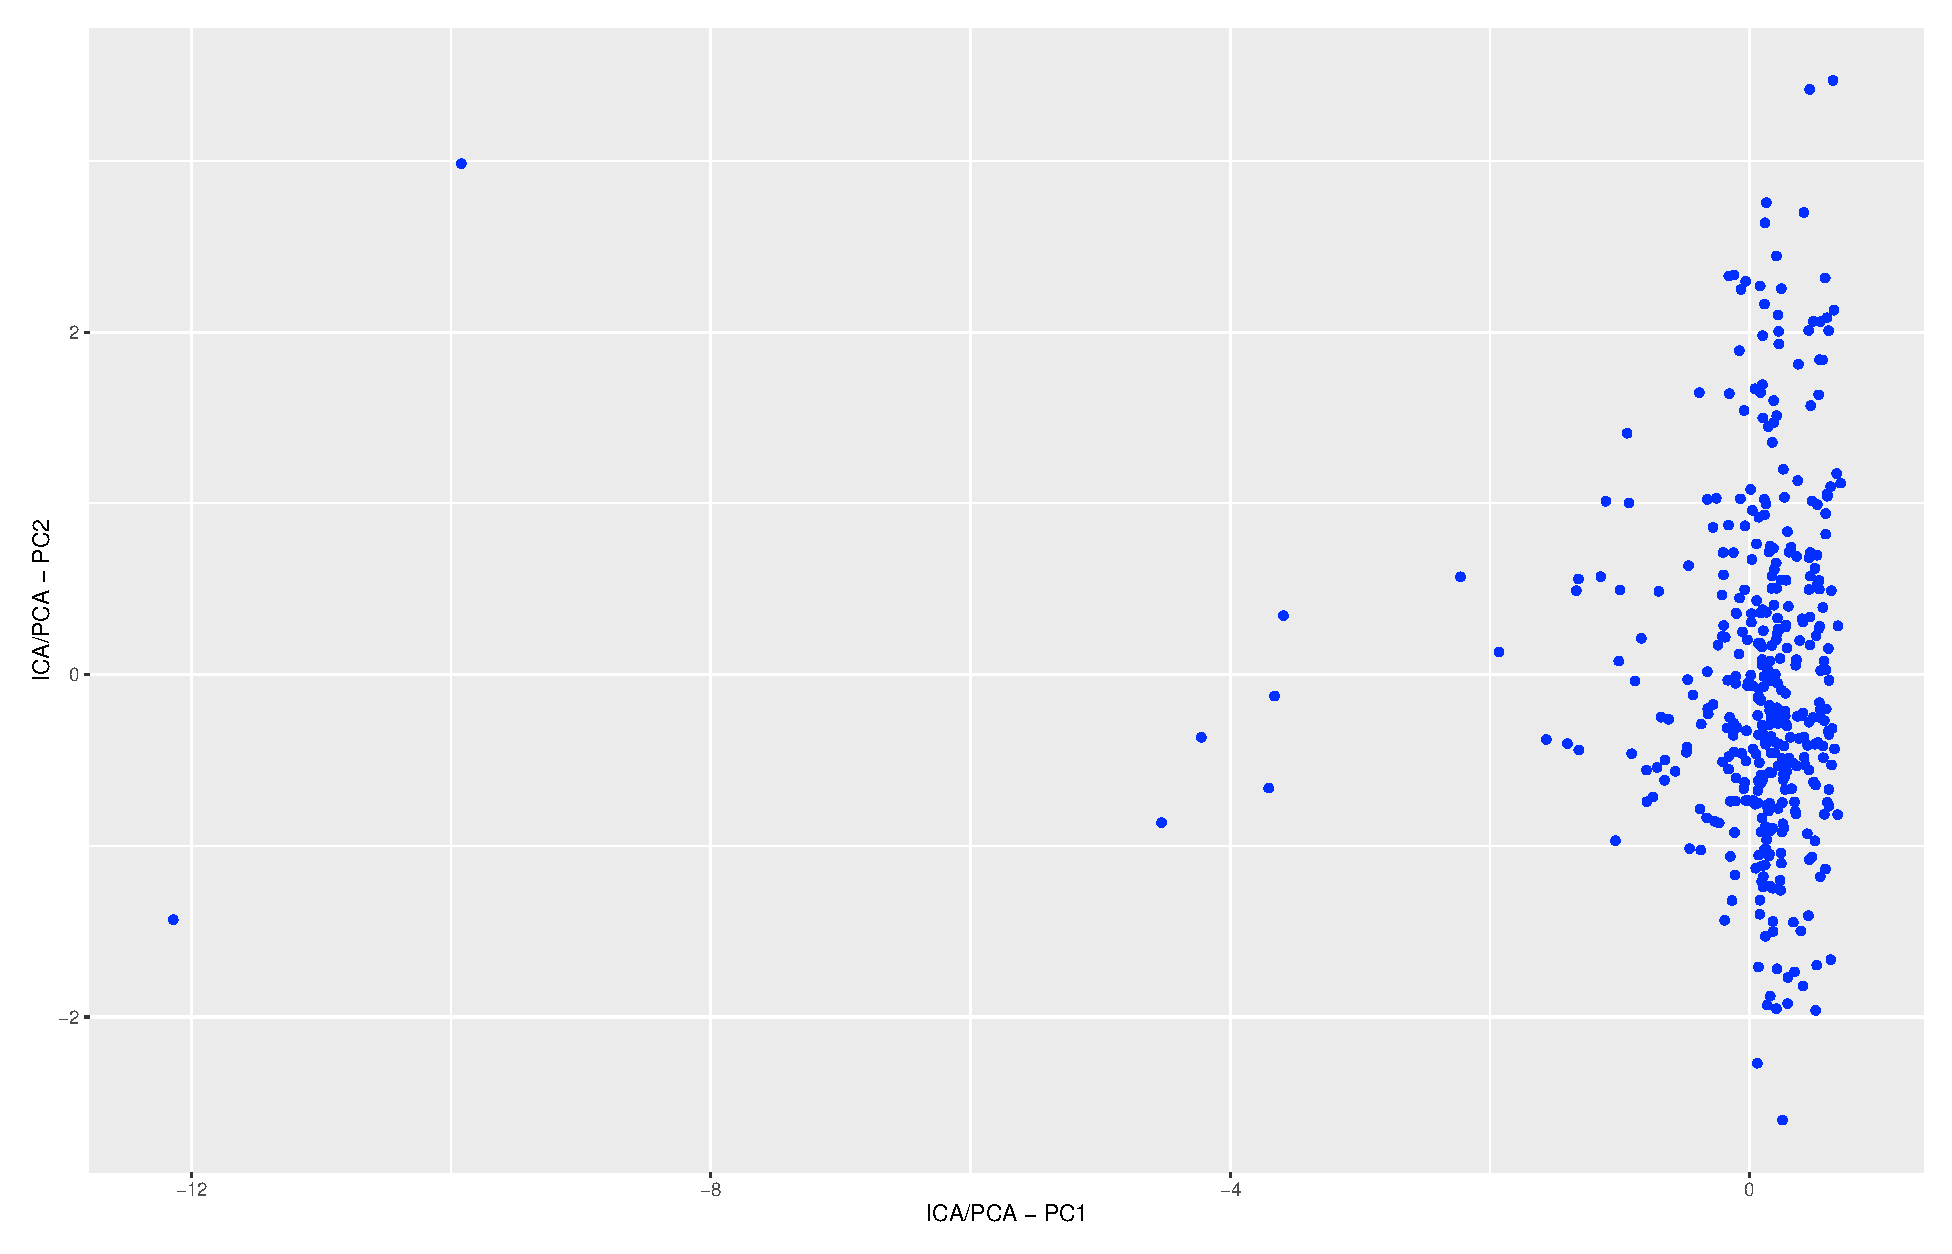
\includegraphics[width=\textwidth]{figures/A2_icascore.eps}
    \end{figure}

    The score distribution is similar to the PCA analysis but with a different magnitude and mirrored Y-values. This could be explained by the analysis switching feature space.

    We perform a \emph{principal component regression} analysis with \emph{cross validation} in order to examine the number of components that should be selected for our model. The result can be observed in figure~\ref{fig:icascores}

    \begin{figure}[H]            
    \centering
    \caption{Mean squared predicted error over number of components}
    \label{fig:viscosity}
    \includegraphics[width=\textwidth]{figures/A2_viscosity.eps}
    \end{figure}

    We can observe from the figure how the MSEP is high when few components are selected and how the mean squared error drastically decreases around 8 components. The number of components with the lowest mean squared error is around 20. The most reasonable number of components would be around 20.
    \newpage
    \section{Appendix: A - Code assignment 1}

    \lstinputlisting[caption=Code for assignment 1,
    label={code/assignment1.r},
    breaklines=true]
    {code/assignment1.r}

    \section{Appendix: B - Code assignment 2}

    \lstinputlisting[caption=Code for assignment,
    label={code/assignment2.r},
    breaklines=true]
    {code/assignment2.r}

    \end{document}
